\documentclass[border=6pt]{standalone}
\usepackage{fontspec,xeCJK,amsmath,amssymb,tikz,graphicx}\setmainfont{Arial}\setCJKmainfont{PingFang SC}\usetikzlibrary{arrows.meta}
\definecolor{ink}{HTML}{203340}\definecolor{teal}{HTML}{147E91}\definecolor{pale}{HTML}{EEF6F6}\definecolor{warm}{HTML}{FFF4E5}
\begin{document}\begin{tikzpicture}[x=1cm,y=1cm,every node/.style={text=ink,font=\fontsize{11}{14}\selectfont},box/.style={rounded corners=6pt,draw=teal!30,fill=white},arr/.style={-{Stealth},thick,teal}]
\path[use as bounding box](0,0)rectangle(11,30);\fill[pale](0,0)rectangle(11,30);
\node[font=\fontsize{21}{25}\selectfont\bfseries]at(5.5,29.2){DreamerV3：学世界，再练行动};\node[text=teal]at(5.5,28.5){Nature 2025｜同一算法配置，各任务独立学习};
\draw[box](.3,22.6)rectangle(10.7,28);\node[anchor=west,font=\bfseries\large]at(.6,27.4){A　真实交互与经验｜Main、Methods};
\node at(3.2,25.9){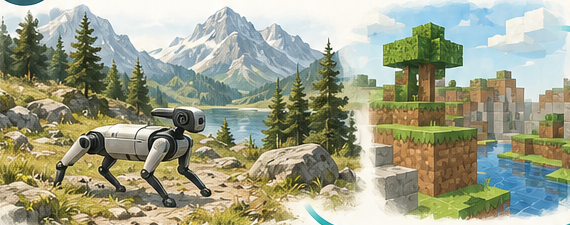
\includegraphics[width=5cm]{environment-art.png}};\node at(8.2,25.9){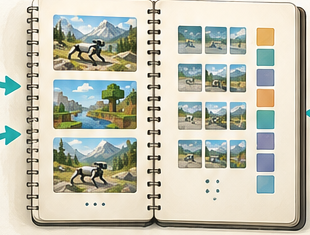
\includegraphics[width=2.7cm]{memory-art.png}};
\draw[arr](5.6,25.9)--(6.6,25.9);\node at(5.5,24.3){环境产生 $(x_t,a_t,r_t,c_t)$，存入 replay};\node at(5.5,23.4){部署：编码实际观察 → actor 出手 → 环境反馈};
\draw[box](.3,15.2)rectangle(10.7,22.2);\node[anchor=west,font=\bfseries\large]at(.6,21.6){B　学习 RSSM｜World model learning};
\node[box,text width=3.2cm,align=center]at(2.6,20.2){真实 $x_t$ + 记忆 $h_t$\\后验 $q(z_t|h_t,x_t)$};\node[box,text width=3.3cm,align=center]at(8,20.2){过去 $h,z,a$ → $h_t$\\先验 $p(z_t|h_t)$};
\draw[arr](4.3,20.2)--node[above]{KL}(6.2,20.2);\node at(5.5,18.8){$s_t=[h_t,z_t]$：连续记忆 + 离散随机状态};
\node at(5.5,17.9){状态 → 图像/向量重构、奖励 $r$、继续概率 $c$};\node at(5.5,17){训练 $\phi$：预测误差 + 动力学 KL + 表征 KL};\node at(5.5,16.1){平衡权重 $1/1/0.1$；free bits；1\% 均匀混合};
\draw[box,fill=warm](.3,7.6)rectangle(10.7,14.8);\node[anchor=west,font=\bfseries\large]at(.6,14.2){C　想象里练策略｜Critic、Actor learning};
\node[box,text width=2cm,align=center]at(2,12.8){replay 状态\\$s_t$};\node[box,text width=2.4cm,align=center]at(5.4,12.8){actor $\pi_\theta$\\选动作 $a_t$};\node[box,text width=2.6cm,align=center]at(9,12.8){世界模型先验\\下个状态 + $r,c$};\draw[arr](3.1,12.8)--(4.1,12.8);\draw[arr](6.7,12.8)--(7.6,12.8);
\draw[arr](9,12)--(9,11.2)--(2,11.2)--(2,12);\node[fill=warm]at(5.5,11.2){抽象状态展开 $T=16$，无需解码图像};
\node at(5.5,10.2){critic $\psi$：估计更远的回报 → $\lambda$-return};\node at(5.5,9.3){actor $\theta$：归一化优势 + 熵，REINFORCE 更新};\node at(5.5,8.4){世界模型提供训练轨迹；部署无需在线树搜索};
\draw[box](.3,.3)rectangle(10.7,7.2);\node[anchor=west,font=\bfseries\large]at(.6,6.6){D　把量纲稳住，再看证据};
\node at(5.5,5.5){Robust predictions：symlog + symexp two-hot};\node at(5.5,4.5){Evaluation：跨域、Minecraft、消融、扩展};\node at(5.5,3.5){Methods：block GRU、LaProp、replay与环境协议};\node[text width=9.4cm,align=center]at(5.5,2.1){文章路线：引言提问 → B 状态学习 → C 回报与动作\\→ D 数值稳定和实验 → 相关工作、结论、实现};\node[font=\fontsize{10}{12}\selectfont]at(5.5,.9){实线表示信息流；参数训练与部署路径分别见 A/B/C};
\end{tikzpicture}\end{document}